% Editable source for probe_pipeline.pdf, written by make_figures.py
\documentclass[border=6pt]{standalone}
\usepackage{tikz}
\usetikzlibrary{positioning,arrows.meta}
\begin{document}
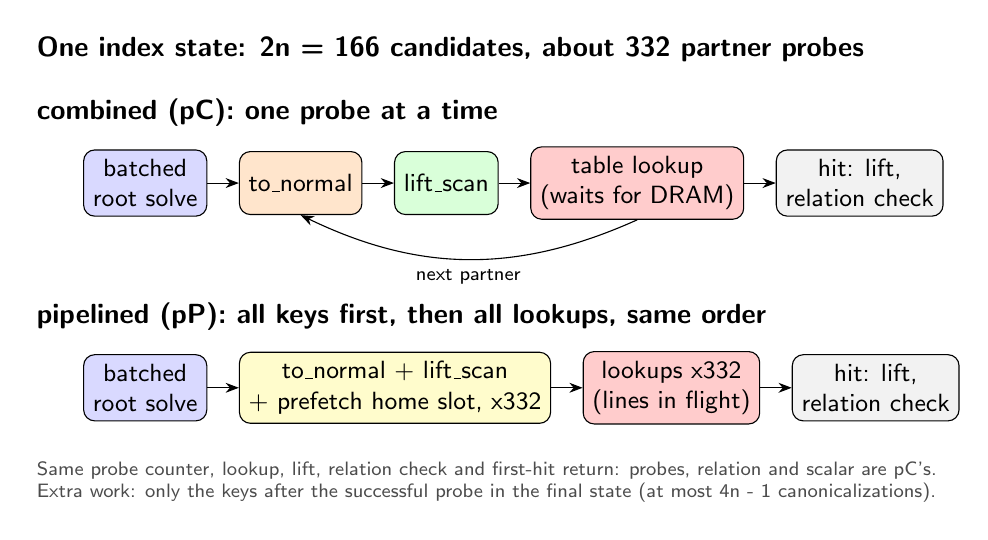
\begin{tikzpicture}[font=\sffamily\small, b/.style={draw, rounded corners, minimum height=0.8cm, align=center},
                    >={Stealth}]
\node[anchor=west,font=\sffamily\bfseries] at (-0.2,2.1) {One index state: 2n = 166 candidates, about 332 partner probes};
\node[anchor=west,font=\sffamily\bfseries] at (-0.2,1.3) {combined (pC): one probe at a time};
\node[b, fill=blue!15] (r1) at (1.3,0.4) {batched\\root solve};
\node[b, fill=orange!20, right=0.4 of r1] (c1) {to\_normal};
\node[b, fill=green!15, right=0.4 of c1] (k1) {lift\_scan};
\node[b, fill=red!20, right=0.4 of k1] (l1) {table lookup\\(waits for DRAM)};
\node[b, fill=black!5, right=0.4 of l1] (h1) {hit: lift,\\relation check};
\draw[->] (r1) -- (c1); \draw[->] (c1) -- (k1); \draw[->] (k1) -- (l1); \draw[->] (l1) -- (h1);
\draw[->] (l1.south) to[bend left=25] node[below,font=\sffamily\scriptsize] {next partner} (c1.south);
\node[anchor=west,font=\sffamily\bfseries] at (-0.2,-1.3) {pipelined (pP): all keys first, then all lookups, same order};
\node[b, fill=blue!15] (r2) at (1.3,-2.2) {batched\\root solve};
\node[b, fill=yellow!20, right=0.4 of r2] (k2) {to\_normal + lift\_scan\\+ prefetch home slot, x332};
\node[b, fill=red!20, right=0.4 of k2] (l2) {lookups x332\\(lines in flight)};
\node[b, fill=black!5, right=0.4 of l2] (h2) {hit: lift,\\relation check};
\draw[->] (r2) -- (k2); \draw[->] (k2) -- (l2); \draw[->] (l2) -- (h2);
\node[anchor=west,font=\sffamily\scriptsize,text=black!70,align=left] at (-0.2,-3.4) {Same probe counter, lookup,
lift, relation check and first-hit return: probes, relation and scalar are pC's.\\ Extra work: only the keys after
the successful probe in the final state (at most 4n - 1 canonicalizations).};
\end{tikzpicture}
\end{document}
